% RMIT University School of CS&IT
% Minor thesis template
% S.M.M. (Saied) Tahaghoghi, 2004
\documentclass[11pt,twoside]{report}
\usepackage{a4wide,caption,epsfig,fancyheadings,url}
\usepackage[colorlinks,citecolor=blue,urlcolor=blue,bookmarks=false,hypertexnames=true]{hyperref}
\usepackage{float}
\usepackage{capt-of}
\usepackage{amsmath}
\usepackage{xcolor}
\usepackage[linesnumbered,ruled]{algorithm2e}
\usepackage{multirow}
\usepackage{longtable}
\usepackage{ragged2e}
\usepackage{array}
    \newcolumntype{P}[1]{>{\centering\arraybackslash}p{#1}}
    \newcolumntype{M}[1]{>{\centering\arraybackslash}m{#1}}

%%% Coloring the pseudocode comment as blue
\newcommand\mycommfont[1]{\footnotesize\ttfamily\textcolor{blue}{#1}}
\SetCommentSty{mycommfont}

\SetKwInput{KwInput}{Input}
\SetKwInput{KwOutput}{Output}

% Place the correct values here
%Set to the original submission date when submitted amended thesis
\newcommand{\SubmissionDate}{\today}
\newcommand{\student}{Qi Xiong}
\newcommand{\supervisor}{Hai Dong}
\newcommand{\topic}{Knowledge Graph Neural Network based Github repository recommendation}
\newcommand{\school}{School of Computing Technologies}
\newcommand{\program}{Masters of Information Technology}
\newcommand{\institution}{RMIT University}

% Use the remark command to highlight text for discussion
\newcommand{\remark}[1]{{\bf \em [\marginpar{$\Leftarrow$}#1]}}

\renewcommand{\leftmark}{\student}
\renewcommand{\rightmark}{\topic}
\renewcommand{\headrulewidth}{0pt}
\setlength{\parindent}{0pt}
\setlength{\parskip}{1.5ex plus 0.3ex}

% This is the line spacing - set to 2 for draft submission to
% supervisor, 1.3 for the final submission
\renewcommand{\baselinestretch}{1.00}

\renewcommand{\captionfont}{\it}
\raggedbottom
\graphicspath{ {./Figs/} }

%For Natbib Author, year citation format
% - the opening bracket symbol, default = (
% - the closing bracket symbol, default = )
% - the punctuation between multiple citations, default = ;
% - the letter n for numerical style, or s for numerical superscript
%   style, any other letter for author year, default = author year;
% - the punctuation that comes between the author names and the year
% - the punctuation that comes between years or numbers when common author lists are suppressed (default = ,);
% \bibpunct{[}{]}{;}{a}{,}{;}


\begin{document}

\title{{\Large\bf \topic}}
\author{
A minor thesis submitted in partial fulfilment of the requirements for the degree of
\\\program\\*[10mm]
%\epsfig{figure=Figs/rmit-coa.epsf,width=5cm}
\\\student
\\\school
\\STEM College
\\\institution
\\Melbourne, Victoria, Australia
}
\maketitle
\thispagestyle{empty}

\chapter*{Declaration}

This thesis contains work that has not been submitted previously, in
whole or in part, for any other academic award and is solely my
original research, except where acknowledged.

This work has been carried out since July 2021, under the
supervision of {\supervisor}.

\paragraph{}
\vspace{5cm}\noindent \\\student \\
\school\\
\institution\\
\SubmissionDate

\pagenumbering{roman}

\chapter*{Acknowledgements}

I would like to acknowledge and express my warmest thanks to my supervisor Hai Dong for his patience and support. His support on computing resources helped me overcome the obstacle in which my laptop is too old and slow for doing the research. His valuable guidance and advice carried me through the writing of the thesis.

I would also like to extend my thanks to the GH Archive project for open sourcing their data set of the public GitHub activities of developers and repositories. The data set provides the most similar use cases in real situations and is ideal for the research of recommending projects.

I would also like to extend my thanks to my fellow students for sharing their ideas, suggestions and experiences in doing minor thesis projects.

Finally, I thank my families and friends for their continuous help and supports.

{
    \hypersetup{linkcolor=black}
    \tableofcontents
    \listoffigures
    \listoftables
}

\pagenumbering{arabic}

\chapter{Abstract}
With the flourishing of the open source communities, the demands of GitHub repositories recommendation cannot be ignored. Many studies have come up with various recommender systems to recommend GitHub repositories to users. However, none of them can deal with data sparsity and cold start issues. To deal with those issues, we proposed a knowledge graph neural network based approach that takes side information into consideration. We found that the performance of our approach overwhelmed the state of the art models in a data set with high data sparsity.

\chapter{Summary}
We introduced the GitHub platform, knowledge graph neural network, side information in the introduction section and our research goal in the introduction section. We then review the literature in the related research field. The reviewed literature was classified into 4 categories that are "Recommender systems", "Graph neural networks", "Knowledge graph neural networks" and "Recommender systems for GitHub repositories". After reviewing the literature, we listed the problem formulation and detailed the design of our solution to the problem in the method section. The solution contains the framework of the model, which we proposed to solve the problem, and the neural network design, which was used as the prediction function of the model. The result and discussion section talked about the experiment result and evaluation of our model. We compared our model with 2 existing models in a data set with high data sparsity. We found that the performance of our model overwhelmed the baseline models. We also compared the 2 existing models with a random recommendation model. This is to prove that the 2 existing models can work in this data set so that the comparison with our model is meaningful. The result turned out that the performance of the 2 existing models surpassed the random recommendation model significantly which means they worked in this data set. Based on the fact that our model significantly outperforms the baseline models, we drew the conclusion that our model can deal with data sparsity and cold start issues.

\chapter{Introduction}
\section{Background}
GitHub \footnote{https://github.com} is an open-source community that enables developers to manage their repositories via a version control system named Git \footnote{https://git-scm.com/}. Developers can also share their projects and contribute to other developers’ projects in this community.

The recommender system for GitHub repositories is important. Developers tend to find repositories that are similar to the ones they are working on to find functions or ideas which can be reused. Although the search engine provided by GitHub can help find similar repositories, it is always not accurate because it only uses the title of repositories rather than the whole details according to \cite{xu_repersp_2017}. While recommender systems can recommend the most relevant repositories to users based on the preference of users.

\textit{Most recommender systems have data sparsity and cold start issues.} Due to the long tail effect, few popular items have the most ratings while lots of others have fewer ratings. As a result, the constructed user-item matrix is sparse. It is inefficient for a model to deal with a sparse matrix. If a user does not rate any items, then it is hard for the recommender system to recommend items to that user. This is the cold start issue. Because in the beginning, there are always few ratings. Researchers have proposed various approaches to tackle these issues.

One of the approaches is to take the side information \cite{jonschkowski_patterns_2016} into consideration. Side information is the data that is outside of the input and output data set of a machine learning system and can provide some useful clues to the machine learning system. For a repository recommender system, the relationships between users and repositories can be used as side information.

Side information can be efficiently integrated into a knowledge graph neural network (KGNN). KGNN is a neural network that takes inputs of a knowledge graph (KG). The neural network can learn the relationships between nodes through the connections in a KG.

With more information that can be used, a recommender system can fight against data sparsity and cold start issues. The improvements are promising according to \cite{zhang_knowledge_2020} which applied side information and knowledge graph neural network to mobile APP recommendations.

Many existing works have proposed various GitHub recommender systems. \textit{But none of them can deal with the cold start problem because they ignored the use of the side information for the recommender system.}

This thesis presented a knowledge graph neural network based model to recommend Github repositories to developers. The performance and the ability to fight against the data sparsity and cold start issues are promising compared with traditional recommender systems. The project of this thesis was open sourced on GitHub \footnote{https://github.com/qinqin65/GitHub-Repo-RS}.

\section{Motivation}
\textit{There is no research in applying KGNN in recommending GitHub repositories while KGNN has the potential to bypass the data sparsity and cold start issues} \cite{mansur_review_nodate}. The recent studies on the GitHub repositories recommender system are based on traditional approaches such as collaborative filtering that are prone to suffer from data sparsity and cold start issues. \textit{For solving those issues, this thesis explores the idea of using the KGNN to recommend GitHub repositories.}

\textit{There is various side information that can be used to build the KGNN based GitHub repositories recommender system.} Users’ behaviours such as "star", "pull" and "fork" (see \ref{fig:watch_star_fork}) can be regarded as side information that indicates the fact that some users are interested in some repositories. Repositories' programming languages (see \ref{fig:programming_languages}) can also be considered as side information that guides the recommender system to recommend the repository to the user with the same programming language preference. Those side information can help the KGNN model to achieve the expected outcome.

\begin{figure}[H]
    \centering
    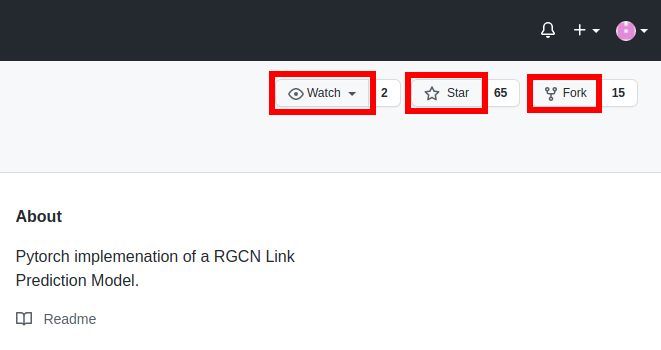
\includegraphics[scale=0.4]{watch_star_fork.png}
    \caption{The watch, star and fork behaviours}
    \label{fig:watch_star_fork}
\end{figure}

\begin{figure}[H]
    \centering
    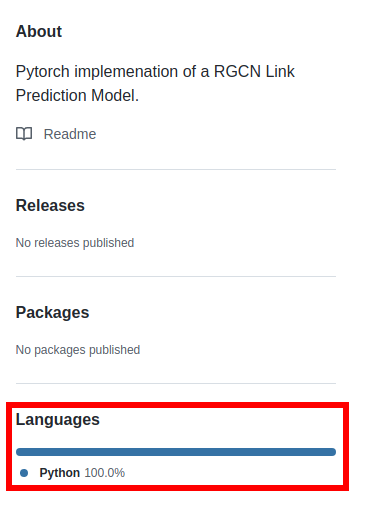
\includegraphics[scale=0.4]{programming_languages.png}
    \caption{Programming languages}
    \label{fig:programming_languages}
\end{figure}

\section{Research questions}
This research aims to propose a KGNN based recommender system for GitHub repositories with high performance and the ability to solve data sparsity and cold start issues by using side information.

Based on this aim, we came up with the below research questions.

\begin{enumerate}
    \item RQ1: What hyperparameter values can make the KGNN model achieve the best performance?
    \item RQ2: Can the performance of the KGNN based repositories recommender system surpass the existing ones?
    \item RQ3: Can the KGNN based repositories recommender system mitigate the data sparsity and cold start issues?
\end{enumerate}

\chapter{Literature review}
\section{Overview}
In this chapter, we reviewed related works in the area of recommender systems, graph neural networks, knowledge graph neural networks and recommender systems for GitHub repositories that are relevant to our research problem.

\section{Recommender systems}
According to \cite{mansur_review_nodate, park_literature_2012}, current recommendation approaches can be classified into three categories: collaborative filtering (CF), content based recommendation, hybrid recommendation. CF can be further classified into memory based and model based approaches. Memory based CF does all calculations in the memory. If it calculates the similarities (i.e., similar in preferences) between users and recommends a user's liked items to his or her similar users who do not know the item, Then it is a user based CF. If it calculates the similarities (i.e., similar in descriptions) between items and recommends an item to users who liked its' similar items, then it is an item based CF. Model based CF recommends items by designing a model which takes users and items as inputs. The model often projects users and items into the same latent space in which similar users and items are close to each other. The output layer of the model often reconstruct the relationship between users and items from the latent space and make predictions on the ratings for unknown user-item pairs. Content filtering calculates the similarities (i.e., similar in contents) between items and recommends an item to a user who liked its' similar items. The hybrid recommendation is a combination of those recommendation approaches.

\section{Graph neural networks}
Graph neural network (GNN) was proposed by \cite{gori_new_2005, scarselli_graph_2009} to learn patterns from graph data that traditional machine learning models cannot handle. The idea is aggregating the state (i.e., a state can be the data represented by a node) of neighbour nodes for each node in the graph using an aggregating function. The aggregating function is restricted to be a contraction mapping for the state of each node. Based on the Banach theorem, the output of the aggregating function is unique regardless of the aggregating order. The state is then inputted to an output function to produce an output. The aggregating function and output function can be neural networks. Based on these ideas, the patterns can be distilled from graph data no matter what order and structure the graph changes. GNN has many successful applications such as learning molecular fingerprints \cite{duvenaud_convolutional_2015}.

The applications of GNN in recommender systems have demonstrated great success as well. Because the data in a recommender system can be represented as a graph structure and GNN are very good at handling connections between nodes according to \cite{wu_graph_2020}. Especially in social recommendations, users and their friends can form a graph. Users’ interaction with items can also form a graph. Fan et al. came up with an approach named “GraphRec” which is based on this fact \cite{fan_graph_2019} and proved that the harness of the relationship between user and user, user and item plays an important role in improving the performance of the recommender system. A session that contains a series of events of interaction between a user and items can also be presented in a GNN model and make predictions about the next event such as which item the user will most likely click. This is classified as a session-based recommendation and plays an important role in web services according to \cite{xu_graph_2019}. The GC-SAN model which makes use of the self-attention algorithm was proposed to identify the transitions of nearby items in a session \cite{xu_graph_2019}.

Most GNN models use low dimensional embedding to represent node features to make them more efficient. However, they still need to iterate all nodes in a graph to learn embeddings. It makes the GNN model very hard to scale to a large data set. Hamilton \cite{hamilton_inductive_2018} proposed the GraphSage model to solve this problem by uniformly sampling neighbour nodes and thus reduce the number of nodes to calculate \cite{hamilton_inductive_2018}. Also, GraphSage can be applied to inductive learning such as predicting embeddings for future unseen nodes.

The use of GNN in recommendation can be classified as the general recommendation and sequential recommendation \cite{wu_graph_2020}. The general recommendation can be powered by Knowledge Graph.

\section{Knowledge graph neural networks}
Knowledge Graph neural network is a subclass of GNN and has gained focus in the field of recommender systems. The side information can be presented in a knowledge graph and can be integrated into a Graph neural network to learn additional knowledge and the performance can be improved accordingly. Zhang et al. \cite{zhang_knowledge_2020} proposed a knowledge graph based approach to recommend mobile Apps and shows promising improvements in performance.

Traditional recommender systems have problems of cold start and data sparsity \cite{zhang_knowledge_2020, mansur_review_nodate, wu_graph_2020} which makes recommendation much difficult in the beginning. Some researchers make use of the side information to help the recommender system to make decisions to solve this problem. The more side information is used the more accurate the recommender system can achieve. There are various types of side information such as the high order relations of items (connect items with two or more linked attributes) \cite{wang_kgat_2019} and semantic information of user-item interactions \cite{wang_knowledge_2019} was explored by researchers. They all show a promising performance according to their papers.

According to \cite{guo_survey_2020}, knowledge graph based recommender systems can be classified into three categories that are embedding-based, connection-based and propagation-based. The most broadly used embedding-based approach projects the nodes and edges of a graph into a lower dimension space in which linked nodes are close to each other. This approach can scale to a large graph but it cannot capture the connection pattern between nodes. The connection-based approaches mine the pattern of connections in a graph. This approach can use the pattern of connections of a graph to guide the recommendation but paths of the connections need to be specified manually. The propagation-based approach combines the advantages of embedding and connection based approaches by aggregating embeddings of neighbour nodes and edges to the current node. This approach can achieve more personalized recommendations but it is hard to scale to a large graph because of the heavy computation of the aggregating process. This disadvantage can be mitigated by using sampling methods.

Knowledge graph based recommender systems can also be explainable according to \cite{guo_survey_2020}. This is achieved by using an attention mechanism. The attention network gives each relation of a graph a weight. Thus the significance of each component is visible and can be used to explain the reason for the recommendation.

While numerous studies show that the advantage of KGNN and the use of side information, there is no study (to my best knowledge) focused on the research of applying this strategy in recommending GitHub repositories. This proposal will be the first one to try this kind of approach.

% \section{Side information}

\section{Recommender systems for GitHub repositories}
The memory based CF model is a mostly used approach in recommending Github repositories. It calculates the similarity between developers and the similarity between repositories. Various preferences such as expertise, technique stacks and behaviours (i.e., star, folk and create) are used to measure the similarity between developers. Repositories' documents such as the readme file and source code are used to measure the similarity between repositories. Some research also take programming languages into consideration \cite{inka_open_2018, sun_personalized_2018}. Most papers determine similarities between repositories by calculating TF-IDF vector space and then calculate cosine distance or Pearson correlation coefficient \cite{mansur_review_nodate, kim_sequential_2021}. After calculating similarities, it defines the ratings for each developer and repository pair. Most papers define the rating by encoding user behaviours into a score coding such as 2 for “star”, 5 for “folk” and 10 for “create” with the higher score standing for the higher weight. Then, it uses various collaborative filtering techniques to recommend repositories.

The second most used approach is a model based approach such as Bayesian personalized ranking matrix factorization (BPRMF) \cite{jiang_open_2017} and Constrained GCN model \cite{shao_paper2repo_2020}. In this kind of approach, users’ behaviour (star, folk and create) and repositories’ documents (readme file and source code) are encoded and represented as a matrix factorization \cite{jiang_open_2017}. Then the task is to search for the best matrix factors to minimize the recommendation error. The sequential recommendation, which includes approaches like gated recurrent units for recommendation (GRU4Rec) and DNN based Caser and SASRec methods \cite{kim_sequential_2021}, are also promising. Kim et al. \cite{kim_sequential_2021} tested and compared those approaches in their work \cite{kim_sequential_2021}.

An approach proposed by \cite{zhang_detecting_2017} are based on some assumptions. For example, if a user stars a repository then the user is interested in that kind of repository. Some assumptions may not be reasonable. For example, if the time gap of two repositories starred by a user is short, then the two repositories are similar. A developer usually stars many non-similar repositories in a short time because they are both important for his or her project. The paper still claims a sound performance according to \cite{zhang_detecting_2017}. \cite{xu_repersp_2017, sun_personalized_2018, zhang_detecting_2017} only tested limited categories of repositories. For example, Vim-jp, Formidable and Harvest-hq. \cite{sun_personalized_2018} only test Java related repository because it relies on the Java API usage pattern to detect similarities \cite{zhang_detecting_2017}. The performance of those models in real situations may not be as good as the papers presented.

Above all, these studies used limited information and data set to build and evaluate their models. It is because the traditional approaches have limitations in using side information. According to the table \ref{tab:literature_review_matrix}, \cite{xu_repersp_2017,inka_open_2018,sun_personalized_2018,zhang_detecting_2017} used a TF-IDF based collaborate filtering approach to recommend repositories. \cite{guendouz_recommending_2015} used a clustering approach to recommend repositories. Those 2 approaches are limited in using side information and prone to suffer from data sparsity. \cite{liu_recommending_2018} used a neural network approach that can use side information such as "last commit time". However, the structure of the neural network, which takes all the repositories to be recommended as inputs, makes it difficult to work in real situations. \textit{Our approach will be focused on recommending repositories to users and incorporating side information into a KGNN to solve data sparsity and cold start issues.}

\begin{center}
    \captionof{table}{Literatures of GitHub recommendation}
    \begin{longtable}{M{0.1\linewidth}M{0.4\linewidth}M{0.2\linewidth}M{0.2\linewidth}}
    \hline
    Literature & Method & Deal with data sparsity & Deal with cold start \\
    \hline
    \cite{xu_repersp_2017} & \justifying Represent the user's behaviour in the form a user-repository matrix, then calculate the similarity (TF-IDF and cosine distance) of repositories by considering their documents and source code, then generate and recommend the top K similar repositories. & N/A & N/A \\
    \hline
    \cite{inka_open_2018} & \justifying Measure the similarity between repositories based on topics (binary vector), programming langauges (binary vector), and readme files (TF-IDF), then recommend the most similar repositories. & N/A & N/A  \\
    \hline
    \cite{sun_personalized_2018} & \justifying Represent the users' behaviour in the form of a matrix UP(user, repository), then calculate the similarity between repositories using documents and source code (calculated TF-IDF vectors), then represent the similarity of repositories as a form of the similarity matrix, then the most similar repositories & N/A & N/A \\
    \hline
    \cite{jiang_open_2017} & \justifying Model the relationship  between users's preference and repositories with a OOCF model, then predict ratings by using the trained model. & N/A & N/A \\
    \hline
    \cite{zhang_detecting_2017} & \justifying Measure the similarity between repositories based on the TF-IDF vector of readme files and the time gap between the starred repositories, then recommend the most similar repositories. & N/A \footnote{"N/A" means not available} & N/A \\
    \hline
    \cite{guendouz_recommending_2015} & \justifying Firstly find the highly similar users, then find the common repositories, then find the highly relevant repositories, finally recommend top k those repositories. & N/A & N/A \\
    \hline
    \cite{liu_recommending_2018} & \justifying Input the repositories to be recommended into a neural network, then train the neural network to output the top K repositories. & N/A & N/A \\
    \hline
    \cite{portugal_gh4re_nodate} & \justifying Use an NLP toolset to get the corpora of repositories, then apply a K-means clustering algorithm to the corpora, then recommended repositories from the same cluster of users & N/A & N/A \\
    \hline
    \end{longtable}
    \label{tab:literature_review_matrix}
\end{center}

\chapter{Methods}
\section{Problem Formulation}
The aim of our work is to predict whether a user will interact with a repository or not. In our design, if a user interacts with a repository, then there is a relationship between them. Since we modelled users, repositories and their relationships in a KG. The relationship is represented as links in the KG. So the problem will be the \textit{link prediction} in which we predict the probability of the existence of links between users and repositories. If a link between a user and a repository exists, then it means that the user will interact with the repository.

We formulated the problem as follows. Given a user $u$, repository $r$ and KG $\mathcal{G}$, learn a prediction function $\hat{y}_r^u=\mathcal{F}(u,r|\mathcal{G},\theta)$ that output the probability $\hat{y}_r^u$ in which the user will interact with the repository. The $\theta$ is the parameters of the prediction function $\mathcal{F}$.

\section{Solution overview}
The framework of the KGNN model was shown in the figure \ref{fig:kgnn_framework}. \textit{There are mainly 4 steps that are KG construction, neural network calculation, prediction and training.} The KG construction step construct the KG from users, repositories and side information by using the Deep Graph Library (DGL) \cite{wang2019dgl}. The neural network calculation step calculates the representation of users and repositories based on the inputs from the KG. The prediction step first calculates the cosine similarity between the representation of users and repositories, then recommends the most similar repositories to users. The training step calculates the loss from the prediction and updates the parameters of the neural network. The steps of neural network calculation, prediction and training form a loop. The parameters are updated and the loss is reduced through the loop.

\textit{There are also some minor processes such as subgraph construction, negative edges sampling and hyperparameters tuning.} The step of the subgraph construction splits the constructed KG into training, validation and testing subgraphs. This is to train and tune the neural network. The step of the negative edge sampling randomly generates false edges, which do not exist in the real data set, between users and repositories. This is to make the neural network learn to avoid folding \cite{xin_folding_2017} in which the neural network may recommend a repository to an irrelevant user. The hyperparameters tuning step tuned the learning rate and dropout rate to maximize the learning performance of the neural network. We will detail them in the following sections.

\begin{figure}[H]
    \centering
    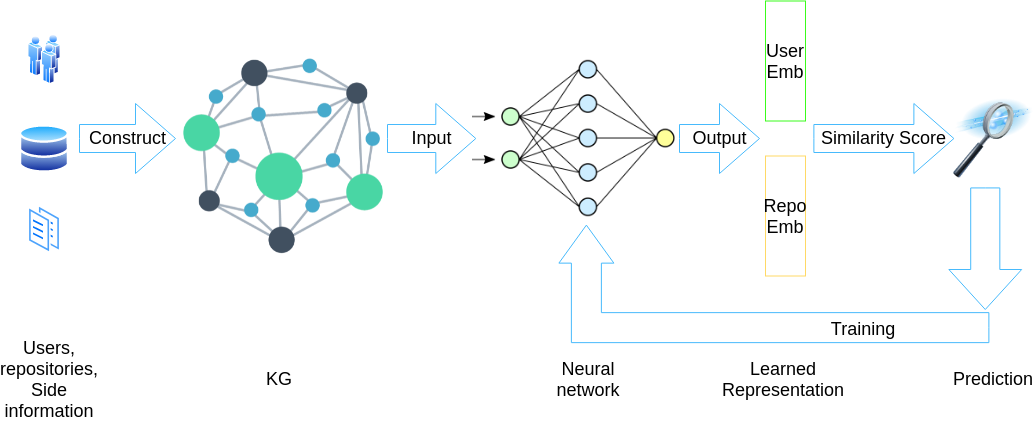
\includegraphics[scale=0.4]{KGCN Overview.png}
    \caption{The framework of the KGNN model}
    \label{fig:kgnn_framework}
\end{figure}

\section{KG construction}
Knowledge graph (KG) can be represented as entity-relation-entity triples $(head, relation, tail)$. The "head" and "tail" are entities. The "relation" is the relationship between the two entities. For example, $(user1, star, repository2)$ means that the user named "user1" starred the repository named "repository2". The relation "star" indicates how a user interacts with a repository. The relation in the entity-relation-entity triples is the same as the edge in the graph structure.

\textit{We explored 2 types of entities and 4 types of relations.} They are shown in the table \ref{tab:edge_types}. "User" means users from GitHub. "Repository" means the repositories that are stored on GitHub. "watch" means a user watches a repository. "star" means a user stars a repository. "fork" means a user forks a repository. "own" means a user is the owner of a repository. 

\begin{center}
    \captionof{table}{Four types of edges}
    \begin{tabular}{l | l | l}
    \hline
    Head & Relation & Tail \\
    \hline
    User & watch & Repository \\
    User & star & Repository \\
    User & fork & Repository \\
    User & own & Repository \\
    \end{tabular}
    \label{tab:edge_types}
\end{center}

Since relation in triples is directed. We added 4 types of reverse relations that are listed in the table \ref{tab:reverse_edge_types}. They are presented in the graph as the reverse edges for the aforementioned 4 types of edges. This is to simplify the process of message passing and aggregation for the 2 types of entities in the training process.

\begin{center}
    \captionof{table}{Four reverse types of edges}
    \begin{tabular}{l | l | l}
    \hline
    Head & Relation & Tail \\
    \hline
    Repository & watched-by & User \\
    Repository & starred-by & User \\
    Repository & forked-by & User \\
    Repository & owned-by & User \\
    \end{tabular}
    \label{tab:reverse_edge_types}
\end{center}

Users and repositories have features such as the users' company name and repositories' description. \textit{We selected 3 features for users and 18 features for repositories as side information.} The selected features are listed in the table \ref{tab:user_features} and \ref{tab:repo_features}.

\begin{center}
    \captionof{table}{The selected features of users}
    \begin{tabular}{l | l}
    \hline
    Feature & Description \\
    \hline
    company & company name \\
    location & users' location \\
    bio & user's introduction \\
    \end{tabular}
    \label{tab:user_features}
\end{center}

\begin{center}
    \captionof{table}{The selected features of repositories}
    \begin{tabular}{l | l}
    \hline
    Feature & Description \\
    \hline
    name & the name of a repository \\
    full\_name & repository's full name \\
    description & repository's description \\
    language & repository's programming language \\
    read\_me & repository's readme files \\
    source\_code & repository's source code \\
    license & repository's open source license \\
    size & the size of the repository \\
    stargazers\_count & number of stars of the repository \\
    watchers\_count & number of watches of the repository \\
    forks\_count & number of forks of the repository \\
    open\_issues & number of oppening issues of the repository \\
    subscribers\_count & number of subscribers of the repository \\
    has\_issues & whether the repository has issues or not \\
    has\_projects & whether the repository has projects or not \\
    has\_downloads & whether the repository has downloads available or not \\
    has\_wiki & whether the repository has wiki function enabled or not \\
    has\_pages & whether the repository has pages or not \\
    \end{tabular}
    \label{tab:repo_features}
\end{center}

The collected users and repositories are numbered starting from 0 and presented in a form of a tuple. The equation \ref{eq:users_tupple} indicates that there are $m$ users. The equation \ref{eq:repos_tupple} indicates that there are $n$ repositories. The tuples for the users and repositories then are inputted into the construction method provided by the DGL to create a graph object. 

\begin{equation}
    (0, 1, 2, ..., m)
    \label{eq:users_tupple}
\end{equation}

\begin{equation}
    (0, 1, 2, ..., n)
    \label{eq:repos_tupple}
\end{equation}

We encoded the features of the users and repositories to numbers since the neural network only accepts numbers. For example, the company name of a user is a string and cannot be inputted into a neural network directly. We convert strings to numbers by using a doc2vec model \cite{le_distributed_nodate} provided by Gensim \cite{rehurek_lrec} that converts variable lengths of strings into a fixed length of vectors. According to \cite{mikolov_efficient_2013}, the converted vectors is the representation of the strings. Some features are already numbers such as the size of the repository. So, no further processes are needed. Some boolean features such as "has\_wiki" are encoded as 1 and 0 which respectively means true and false. The encoded features are then normalized between 0 and 1.

The features of the users and repositories are presented as a matrix in which the rows indicates users or repositories and the columns indicates their features. The matrix \ref{matrix:user_feature} indicates that there are $m$ users and each user has a feature of dimension $n$. The matrix \ref{matrix:repo_feature} indicates that there are $j$ repositories and each repository has a feature of dimension $k$. The 2 matrices are attached to the graph object created above.

\begin{equation}
    \begin{bmatrix}
        1 & 0 & .3 & .5 & ... & n \\
        0 & .4 & 1 & .6 & ... & n \\
        . & . & . & . & ... & n \\
        . & . & . & . & ... & n \\
        . & . & . & . & ... & n \\
        m & m1 & m2 & m2 & ... & n
        \label{matrix:user_feature}
    \end{bmatrix}
\end{equation}

\begin{equation}
    \begin{bmatrix}
        1 & 0 & .3 & .5 & ... & k \\
        0 & .4 & 1 & .6 & ... & k \\
        . & . & . & . & ... & k \\
        . & . & . & . & ... & k \\
        . & . & . & . & ... & k \\
        j & j1 & j2 & j2 & ... & k
        \label{matrix:repo_feature}
    \end{bmatrix}
\end{equation}

\textit{The training, validation and testing subgraph were constructed from the aforementioned heterogeneous graph.} The subgraphs were constructed through edge sampling with a ratio of 60:20:20 for training, validation and testing.

\textit{We sampled negative edges with the amount as the same as the positive edges.} The negative training, validation and testing graph were constructed from those negative edges.

\section{Neural network design}
Figure \ref{fig:kgnn_structure} shows the structure of the KGNN model. The neural network for the knowledge graph contains 3 layers that are the embedding layer, hidden layer and output layer. We designed an embedding layer to learn the low dimensional representation of users and repositories. We used a hidden layer to capture the nonlinear relationships in the data set. The output layer was designed to project the user representations and repository representations into the same space in which the representations of users and repositories are close if they have relationships (i.e., a user stars a repository). 

The embedding layer contains 2 sub single layer neural networks that are used to embed users and repositories. The hidden layer is a graph convolutional network (GCN) \cite{kipf_semi-supervised_2017} layer that contains 4 sub GCN layers respectively for the 4 types of edges. The output of the 4 GCNs of the hidden layer will be aggregated with the sum aggregation. The output layer is also a GCN layer that contains 4 sub GCN layers. The output of the 4 GCNs of the output layer will also be aggregated with the sum aggregation. The output contains learned users' representation and repositories' representation.

\begin{figure}[H]
    \centering
    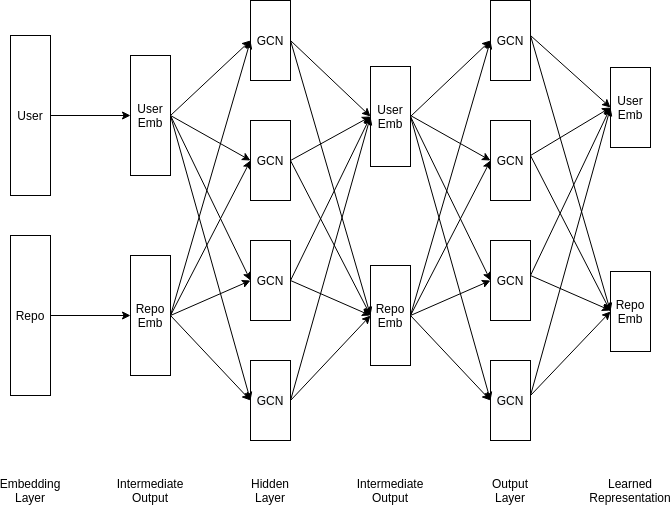
\includegraphics[scale=0.6]{KGCN Structure.png}
    \caption{The neural network structure of the KGNN model}
    \label{fig:kgnn_structure}
\end{figure}

Nodes in the GCN will go through the process of message passing and aggregation with their neighbour nodes to get their new representation. In the process of message passing, every neighbour of a node sends its representation to the current node. In the process of aggregation, the current node aggregates the representation vectors received. We used sum aggregation as the aggregation function. After the aggregation, the result will go through an activation function and calculate the new representation for the current node. The equation \ref{eq:message_passing_aggregation} depicts this process.

\begin{equation}
    h_u^{n+1}=\delta(sum(h_u^n, \sum_{v\in{N(u)}}h_v^n))
    \label{eq:message_passing_aggregation}
\end{equation}

The $h_u$ means the representation of the current node. The $\delta$ means the activation function. The $N(u)$ means the neighbour nodes of the current node. The $h_v$ means one of the neighbour nodes of the current node.

The output representation vectors of the neural network should be similar for nodes that have positive edges and dissimilar for those who have negative edges.

\section{Prediction}
The prediction process uses the learned representation vectors of users and repositories to calculate the similarity score between them. The recommender system then recommends the top $K$ most similar repositories to users.

The similarity score is measured by using cosine similarity. The equation \ref{eq:cosine_similarity} shows how the similarity score is calculated. The $u$ and $r$ means "User" and "Repository". The $h_u$ and $h_r$ means the learned representation of users and repositories.

\begin{equation}
    sim(u, r) = \frac{h_u}{\|h_u\|}\cdot\frac{h_r}{\|h_r\|}
    \label{eq:cosine_similarity}
\end{equation}

\section{Loss function}
To make the neural network learn to output the expected representations, we used a \textit{hinge loss function} as shown in the equation \ref{eq:loss_function}.

\begin{equation}
    l=\frac{1}{m\cdot{e}}\sum_{i=1}^{m}\sum_{j}^{e} max(0, f(n_u, n_v)+\Delta-f(p_u, p_v))
    \label{eq:loss_function}
\end{equation}

The $m$ means the number of types of edges (in this case it is 4). The $e$ means the number of edges. The $f$ means the cosine similarity. The $n_u$ and $n_v$ means the source and destination nodes for the negative edge $j$. The $p_u$ and $p_v$ means the source and destination nodes for the positive edge $j$. The $\Delta$ is the correction parameter that prevents the loss from becoming zero.

\section{Alternaltives}
\subsection{Dense neural network}
We could use a densely connected neural network (DNN) instead of GCN. According to \cite{kipf_semi-supervised_2017}, DNN in a graph learns node specific weight matrices. It is difficult to be scaled to a large graph. While the GNN learns a single weight matrix to handle nodes in a graph. It makes it relatively computational cheap when applying it to a large graph. This is the reason why we chose the GCN as the graph neural network.

\chapter{Results and Discussion}
\section{Experiment overview}
To answer the research questions, we designed an experiment in which the models was evaluated in a data set with high data sparsity. The models include the KGNN model and 3 baseline models. The evaluation metrics include hit rate, MRR and NDCG. We will detail them in the following sections.

The 3 baseline models are TF-IDF model, collaborative filtering model and random recommendation model. The random recommendation model is used to prove that the baseline models are indeed working in this data set with high data sparsity.

To answer RQ1, we tuned the hyperparameters of the KGNN model in this data set to see which hyperparameters can make the KGNN model achieve its best performance.

To answer RQ2, we evaluated the 4 models in this data set with the 3 metrics and compared their performance.

To answer RQ3, we evaluated the 4 models in the data set in which users have at most 1 repository and compared their performance.

\section{Data collection}
The data was collected from GitHub Archive \footnote{https://www.githubarchive.org/} which records activities from developers and repositories via GitHub API \footnote{https://docs.github.com/en/rest} subscriptions. GitHub API was also used in this thesis to collect additional information for developers and repositories such as the programming languages, user introductions, source code and readme files. The collected data set was separated into 60\% for training, 20\% for validation and 20\% for testing.

\section{Data exploration}
The collected data set contains 4417 users and 7054 repositories. There are 42316 interactions (e.g. star, watch and fork) between users and repositories. The scale of the data set is small due to the quota limitations of the developer API provided by GitHub but enough for the experiment.

From the figure \ref{fig:user_repo_dist_hist} and \ref{fig:user_repo_dist_bar}, we can see that most repositories interact with less than 5 users while few of them interact with at most 50 users. It means that the data collected is very sparse. The rating matrix of users and repositories has too many zeros (regard a fork or star behaviour as a rating). The sparsity is 0.062\% for this data set.

\begin{figure}[H]
    \centering
    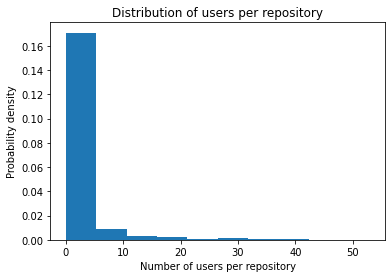
\includegraphics[scale=0.9]{user_repo_dist_hist.png}
    \caption{Hist diagram for the distribution of repositories per user}
    \label{fig:user_repo_dist_hist}
\end{figure}

\begin{figure}[H]
    \centering
    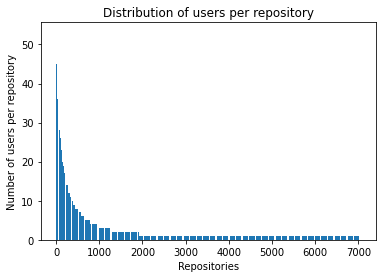
\includegraphics[scale=0.9]{user_repo_dist_bar.png}
    \caption{Bar diagram for the distribution of repositories per user}
    \label{fig:user_repo_dist_bar}
\end{figure}

\section{Training}
\subsection{Evaluation metrics for training}
We use the AUC score to evaluate the training process. The AUC score is calculated as the area under the ROC curve. It has a range of 0 to 1. The higher the score means the better the performance.

\subsection{Training results}
The KGNN was trained with the PyTorch library and Adam optimizer in 100 epochs. We found that the training loss decreased sharply at the beginning and stays stable at around the epoch of 80 (see \ref{fig:training_loss}). However, the validation loss is always lower than the training loss. This is because the dropout behaviour of the neural network is suspended when calculating the validation loss. So, the validation loss can be lower than the training loss. Also, the validation graph has fewer edges than that of the training graph. It leads to fewer positive numbers in the loss and the hinge loss function simply ignores the numbers below 0. 

From the figure \ref{fig:training_loss} and \ref{fig:auc}, we can see that the validation loss does not change too much after 40 epochs and the AUC score decreases after 60 epochs. It indicates that we can stop training at the epoch of around 40 to 60.

\begin{figure}[H]
    \centering
    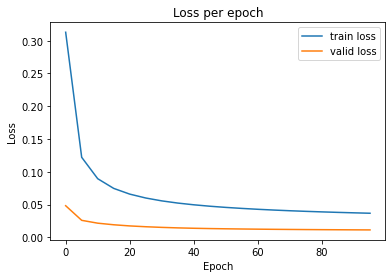
\includegraphics[scale=0.9]{loss.png}
    \caption{The training and validation loss of the KGNN}
    \label{fig:training_loss}
\end{figure}

\begin{figure}[H]
    \centering
    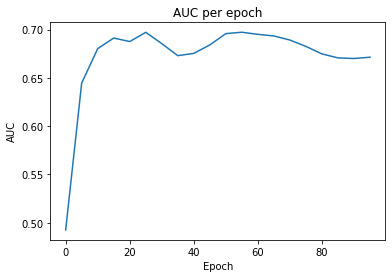
\includegraphics[scale=0.9]{auc.png}
    \caption{The AUC score}
    \label{fig:auc}
\end{figure}

\section{Hyper parameters tuning}
\subsection{Learning rate}
We tuned the neural network with different learning rates. The result can be seen from the figure \ref{fig:auc_learning_rate}. The learning rate of 0.01 can achieve the best result.

\begin{figure}[H]
    \centering
    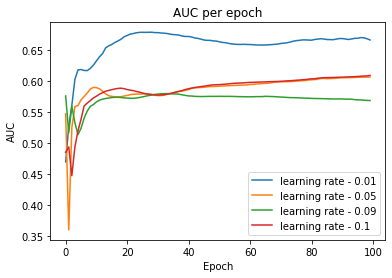
\includegraphics[scale=0.9]{auc_learning_rate.png}
    \caption{The AUC score under different learning rates}
    \label{fig:auc_learning_rate}
\end{figure}

\subsection{Dropout}
\textit{To prevent the model from becoming overcomplicated, we added dropout layers between the embedding layer, hidden layer and out layer.} We tested different dropout rates and found that when the dropout rate is 0.4 the neural network can achieve a better result (see \ref{fig:auc_drop_out_rate}).

\begin{figure}[H]
    \centering
    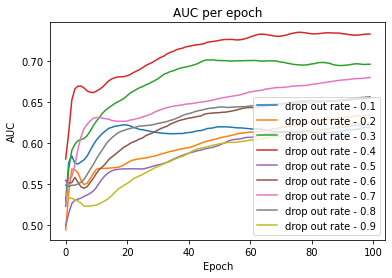
\includegraphics[scale=0.9]{auc_drop_out_rate.png}
    \caption{The AUC score under different dropout rates}
    \label{fig:auc_drop_out_rate}
\end{figure}

\section{Baseline models}
\subsection{TF-IDF approach}
A TF-IDF approach proposed by \cite{xu_repersp_2017,sun_personalized_2018} was used as a baseline model for the evaluation of the KGNN based model. TF-IDF means term frequency and inverse document frequency which calculates the ratio between the frequency of the appearance of a term and the frequency of documents that contains the term. It can be used to measure the similarity between documents. The TF-IDF vectors of documents with a similar topic tend to be similar.

This TF-IDF approach calculates the TF-IDF vectors for readme files and source code for all repositories. Based on those TF-IDF vectors, the 2 similarity matrices between repositories can be constructed (one for the readme files and another one for the source code). The final similarity score between repositories is calculated by combining the 2 matrices using the equation \ref{eq:sim_repositories}. After the calculation of the similarity matrix, the algorithm recommends the most similar repositories to users.

\begin{gather}
    SIM(a,b)=\alpha\cdot{SIM_{readme}(a,b)}+\beta\cdot{SIM_{src}(a,b)}, \\
    s.t.\quad\alpha+\beta=1.
    \label{eq:sim_repositories}
\end{gather}

The $a$ and $b$ are repositories. The $\alpha$ and $\beta$ are hyperparameters meant to control the weight of the 2 types of similarities. They are tuned to 0.9 and 0.1 respectively in this experiment.

\subsection{Collaborate filtering approach}
A collaborative approach \cite{guendouz_recommending_2015} (CF) was also used as a baseline model for the evaluation of the KGNN based model. This approach measures the similarities between users and recommends the most "co-rated" repositories from the most similar users. The similarity measurement is the number of interactions (e.g. the number of stars).

\begin{algorithm}[H]
    \DontPrintSemicolon
    
    \tcc{The u and v are two GitHub users}
    \KwInput{u, v}
    \tcc{The score is measured by the number of common repositories}
    \KwOutput{The similarity score between u and v}

    $count \leftarrow 0$ \newline
    \tcc{$R_u$ is the list of repositories of the user u}
    \ForEach{$r$ in $R_u$}
    {
        \tcc{$R_v$ is the list of repositories of the user v}
        \If{$r$ in $R_v$}
        {
            $count \leftarrow count + 1$
        }
    }
    \Return $count$
    
    \caption{similar}
    \label{alg:similar}
\end{algorithm}

The algorithm \ref{alg:similar} shows the pseudocode of measuring the similarity between users. The algorithm \ref{alg:ratings} shows the pseudocode of calculating the most rated common repositories between similar users. The top k most rated common repositories from the most similar users will be recommended.

\begin{algorithm}[H]
    \DontPrintSemicolon
    
    \tcc{The r is a GitHub repository}
    \KwInput{r}
    \tcc{The rating is measured as the number of interactions between users and repositories}
    \KwOutput{The number of ratings of the repository r}

    $ratings \leftarrow 0$ \newline
    \tcc{The $Users$ is the highly similar users}
    \ForEach{$user$ in $Users$}
    {
        \tcc{The $R_{user}$ is the list of repositories of the user}
        \If{$r$ in $R_{user}$}
        {
            $ratings \leftarrow ratings + 1$
        }
    }
    \Return $ratings$
    
    \caption{number\_of\_ratings}
    \label{alg:ratings}
\end{algorithm}

\subsection{Random recommendation}
Since traditional recommender systems suffer from data sparsity and cold start issues. They may end up in a poor performance during the evaluation. To determine whether they work or not, we used a random recommender as the contrast model. The poor performance models should be at least better than a random recommendation model. The algorithm \ref{alg:random_recommendation} shows the pseudocode of this random recommendation model.

\begin{algorithm}[H]
    \DontPrintSemicolon
    
    \tcc{The user is a GitHub user}
    \tcc{The repositories is a list of Github repositories. The index of the list indicates the number of the repository. The value of 0 indicates that the repository has no relationship with the user}
    \tcc{The k means the k repositories to be recommended}
    \KwInput{user, repositories, k}
    \tcc{The rating is measured as the number of interactions between users and repositories}
    \KwOutput{Top k recommendations}

    \tcc{Remove the repositories with which the user already interacted}
    \ForEach{$r$ in $repositories$}
    {
        \tcc{The $R_{user}$ is the list of repositories of the user}
        \If{$r$ in $R_{user}$}
        {
            $r \leftarrow 0$
        }
    }

    $recommendations \leftarrow choice(repositories[repositories>0], k)$

    \Return $recommendations$
    
    \caption{random\_recommendation}
    \label{alg:random_recommendation}
\end{algorithm}

\section{Evaluation metrics for comparison}
\subsection{Hit rate}
The hit rate measures the ratio between hit repositories and all the repositories recommended. If a recommended repository is on the list of users' repositories, then it means a hit. The higher the ratio means the more accurate the recommendation. It does not consider the ranking order of the relevance of recommended repositories. The equation \ref{eq:hit_rate} shows how this metric is calculated.

\begin{equation}
    HitRate=\frac{R_{hit}}{R_{hit}+R_{missed}}
    \label{eq:hit_rate}
\end{equation}

\subsection{Mean Reciprocal Rank}
While hit rate does not evaluate the ranking order of recommendations, Mean Reciprocal Rank (MRR) evaluates the accuracy of the ranking order of the most relevant recommendation. The equation \ref{eq:mrr} shows how it is calculated. The $Q$ means the total number of queries (each query can be seen as the recommendations for a specific user). The $rank_i$ means the rank of the most relevant recommendation.

\begin{equation}
    MRR=\frac{1}{Q}\sum_{i=1}^Q\frac{1}{rank_i}
    \label{eq:mrr}
\end{equation}

\subsection{Normalized Discounted Cumulative Gain}
Normalized Discounted Cumulative Gain (NDCG) evaluates the quality of the rank of the recommendations. Unlike MRR only evaluates one single item rank of a recommendation, NDCG evaluates the ranks of all the items of a recommendation. The Discounted Cumulative Gain(DCG) and Ideal Discounted Cumulative Gain(IDCG) need to be calculated, then normalized to produce the NDCG score. 

DCG is calculated by summing all the relevance scores, which is discounted by a log function of its position, of the recommendations. In this experiment, the relevance score is defined in the table \ref{tab:relevance_score}. If a recommended repository is in the user's watch list, then it gets a relevance score of 1. The equation \ref{eq:dcg} shows how the DCG is calculated. The $k$ means the number of recommended repositories.

IDCG is the best DCG the recommender system can achieve (like an upper bound). In IDCG, the highest relevance score will rank before the lowest one. Since the relevance score is discounted by their position, so the descending order of the relevance score will achieve the best DCG.

The NDCG is the normalized DCG. The equation \ref{eq:ndcg} shows how it is calculated.

\begin{center}
    \captionof{table}{The definition of the relevance score}
    \begin{tabular}{l | l}
    \hline
    Relation & Relevance score \\
    \hline
    watch & 1 \\
    star & 2 \\
    fork & 3 \\
    own & 4
    \end{tabular}
    \label{tab:relevance_score}
\end{center}

\begin{equation}
    DCG=\sum_{i=1}^k\frac{relevance\_score_i}{log_2(i+1)}
    \label{eq:dcg}
\end{equation}

\begin{equation}
    NDCG=\frac{DCG}{IDCG}
    \label{eq:ndcg}
\end{equation}

\section{Results}
Since the data set is imbalanced (most users have fewer repositories while few users have more than 20 repositories), we split the results into 4 groups based on the number of repositories to study the performance in different groups. The groups are shown in the table \ref{tab:4_groups}. "Group 0 to 5" means that the users in this group have 0 to 5 (not including 5) repositories. If the repositories of the users are less than the designated top $k$, then the recommender will recommend the same amount of repositories of the users.

\begin{center}
    \captionof{table}{4 groups}
    \begin{tabular}{l | l}
    \hline
    No. & Group \\
    \hline
    1 & 0 to 5 \\
    2 & 5 to 10 \\
    3 & 10 to 15 \\
    4 & 15 and over
    \end{tabular}
    \label{tab:4_groups}
\end{center}

To investigate whether the KGNN model can solve the cold start issue, we examed the recommendation performance in users who have only 1 repository. The KGNN model can recommend repositories to users who have no repositories in the training data set once it learns the representation of the users and repositories.

\subsection{Overall performance}
The table \ref{tab:overall_performance} shows the overall performance for top 10, top 15 and top 20 recommendations. The performance of the KGNN model surpassed the baseline models significantly in all the metrics.

The difference in the performance is huge between the KGNN model and the baseline models. The reason is that the other models suffer from data sparsity. The TF-IDF and CF model are based on traditional approaches that are susceptible to data sparsity. \textit{Their performance surpassed the random model significantly which means the 2 models worked but cannot work well when the data is sparse.}

\begin{center}
    \captionof{table}{Overall performance}
    \begin{tabular}{l | l | l | l | l}
    \hline
    Top K & Model & Hit Rate & MRR & nDCG \\
    \hline
    \multirow{4}{*}{10} 
    & KGNN & \textbf{0.73} & \textbf{0.3} & \textbf{0.75} \\
    & TF-IDF & 0.037 & 0.025 & 0.021 \\
    & CF & 0.056 & 0.01 & 0.005 \\
    & Random & 0.002 & 0.001 & 0.000 \\
    \hline
    \multirow{4}{*}{15}
    & KGNN & \textbf{0.73} & \textbf{0.3} & \textbf{0.74} \\
    & TF-IDF & 0.043 & 0.025 & 0.021 \\
    & CF & 0.067 & 0.01 & 0.005 \\
    & Random & 0.002 & 0.001 & 0.000 \\
    \hline
    \multirow{4}{*}{20}
    & KGNN & \textbf{0.75} & \textbf{0.3} & \textbf{0.76} \\
    & TF-IDF & 0.046 & 0.025 & 0.021 \\
    & CF & 0.075 & 0.01 & 0.004 \\
    & Random & 0.004 & 0.001 & 0.001 \\
    \end{tabular}
    \label{tab:overall_performance}
\end{center}

\subsection{Hit rate group performance}
According to the table \ref{tab:hit_rate_group_performance}, the hit rate for the KGNN in "group 15 and above" can reach as high as 0.85 when the top $k$ is 20. The hit rate for "group 0 to 5" is stable and around 0.75. The hit rate for the middle tier (group 5 to 10 and 10 to 15) is quite poor compared with other tiers. The reason is that the number of records of the middle tier is small than that of the "group 0 to 5" which takes up about 80\% of the records. The reason why the "group 15 and above" has a high hit rate may be that the number of records of repositories is large and relatively easy to get hit.

The pattern of performance of the 4 groups of the baseline models is similar to that of the KGNN model. The performance of the KGNN model surpassed other models across the 4 groups.

\begin{center}
    \captionof{table}{Hit rate group performance}
    \begin{tabular}{l | l | l | l | l | l}
    \hline
    Top K & Model & 0 to 5 & 5 to 10 & 10 to 15 & 15 and over \\
    \hline
    \multirow{4}{*}{10} 
    & KGNN & \textbf{0.76} & \textbf{0.59} & \textbf{0.69} & \textbf{0.82} \\
    & TF-IDF & 0.034 & 0.04 & 0.067 & 0.103 \\
    & CF & 0.058 & 0.079 & 0.013 & 0.017 \\
    & Random & 0.002 & 0.000 & 0.003 & 0.004 \\
    \hline
    \multirow{4}{*}{15}
    & KGNN & \textbf{0.75} & \textbf{0.53} & \textbf{0.44} & \textbf{0.42} \\
    & TF-IDF & 0.04 & 0.054 & 0.072 & 0.08 \\
    & CF & 0.069 & 0.091 & 0.017 & 0.015 \\
    & Random & 0.001 & 0.000 & 0.002 & 0.006 \\
    \hline
    \multirow{4}{*}{20}
    & KGNN & \textbf{0.75} & \textbf{0.57} & \textbf{0.68} & \textbf{0.85} \\
    & TF-IDF & 0.044 & 0.054 & 0.083 & 0.068 \\
    & CF & 0.078 & 0.116 & 0.02 & 0.015 \\
    & Random & 0.004 & 0.006 & 0.000 & 0.004 \\
    \end{tabular}
    \label{tab:hit_rate_group_performance}
\end{center}

\subsection{MRR rate group performance}
Based on the table \ref{tab:mrr_group_performance}, the MRR of the group "5 to 10" is the highest for all models and top $k$s. However, the sample size in this group is not large. The reason why this group has the highest MRR is unknown. The MRR of the KGNN model surpassed the baseline models. \textit{It means that the KGNN model is more accurate in ranking the most relevant repository to the right position.}

\begin{center}
    \captionof{table}{MRR group performance}
    \begin{tabular}{l | l | l | l | l | l}
    \hline
    Top K & Model & 0 to 5 & 5 to 10 & 10 to 15 & 15 and over \\
    \hline
    \multirow{4}{*}{10} 
    & KGNN & \textbf{0.28} & \textbf{0.55} & \textbf{0.39} & \textbf{0.33} \\
    & TF-IDF & 0.016 & 0.153 & 0.208 & 0.21 \\
    & CF & 0.01 & 0.067 & 0.022 & 0.022 \\
    & Random & 0.000 & 0.000 & 0.007 & 0.023 \\
    \hline
    \multirow{4}{*}{15}
    & KGNN & \textbf{0.29} & \textbf{0.57} & \textbf{0.41} & \textbf{0.42} \\
    & TF-IDF & 0.017 & 0.159 & 0.209 & 0.204 \\
    & CF & 0.009 & 0.038 & 0.017 & 0.032 \\
    & Random & 0.000 & 0.000 & 0.004 & 0.040 \\
    \hline
    \multirow{4}{*}{20}
    & KGNN & \textbf{0.28} & \textbf{0.55} & \textbf{0.39} & \textbf{0.34} \\
    & TF-IDF & 0.017 & 0.159 & 0.208 & 0.2 \\
    & CF & 0.009 & 0.085 & 0.029 & 0.032 \\
    & Random & 0.001 & 0.012 & 0.000 & 0.011 \\
    \end{tabular}
    \label{tab:mrr_group_performance}
\end{center}

\subsection{NDCG rate group performance}
According to the table \ref{tab:ndcg_group_performance}, the group "15 and over" has the highest NDCG for all models and top $k$s. The NDCG of baseline models does not change too much across different top $k$s. The NDCG of the KGNN model surpassed baseline models significantly. \textit{It means that the KGNN model is more accurate in ranking each repository in a recommendation to the right position.}

\begin{center}
    \captionof{table}{NDCG group performance}
    \begin{tabular}{l | l | l | l | l | l}
    \hline
    Top K & Model & 0 to 5 & 5 to 10 & 10 to 15 & 15 and over \\
    \hline
    \multirow{4}{*}{10} 
    & KGNN & \textbf{0.75} & \textbf{0.68} & \textbf{0.77} & \textbf{0.85} \\
    & TF-IDF & 0.016 & 0.048 & 0.069 & 0.110 \\
    & CF & 0.004 & 0.031 & 0.012 & 0.013 \\
    & Random & 0.000 & 0.000 & 0.003 & 0.006 \\
    \hline
    \multirow{4}{*}{15}
    & KGNN & \textbf{0.75} & \textbf{0.64} & \textbf{0.53} & \textbf{0.56} \\
    & TF-IDF & 0.016 & 0.048 & 0.068 & 0.109 \\
    & CF & 0.004 & 0.018 & 0.011 & 0.015 \\
    & Random & 0.000 & 0.000 & 0.001 & 0.008 \\
    \hline
    \multirow{4}{*}{20}
    & KGNN & \textbf{0.75} & \textbf{0.65} & \textbf{0.75} & \textbf{0.88} \\
    & TF-IDF & 0.016 & 0.048 & 0.068 & 0.111 \\
    & CF & 0.003 & 0.036 & 0.01 & 0.013 \\
    & Random & 0.000 & 0.006 & 0.000 & 0.004 \\
    \end{tabular}
    \label{tab:ndcg_group_performance}
\end{center}

\subsection{Performance of solving the cold start issue}
To test whether the KGNN model can solve the cold start issue, we had a look at the performance of the recommendation in users who have only 1 repository in the test data set. Since there is only 1 repository, so the results of the MRR and NDCG metric are the same as the hit rate metric. We only list the performance of the hit rate in the table \ref{tab:top_1_recommendation}.

\begin{center}
    \captionof{table}{Top 1 recommendation}
    \begin{tabular}{c | l | l}
    \hline
    Top K & Model & Hit rate \\
    \hline
    \multirow{4}{*}{1} 
    & KGNN & \textbf{0.209} \\
    & TF-IDF & 0.011 \\
    & CF & 0.018 \\
    & Random & 0.002 \\
    \end{tabular}
    \label{tab:top_1_recommendation}
\end{center}

The performance of the KGNN model of solving the cold start issue is not promising as solving the data sparsity issue. However, its performance is still significantly better than that of baseline models.

\section{Discussion}
According to the results of the 3 metrics, the KGNN model has the highest performance while other models have an extremely poor performance. The random recommendation model has the poorest performance due to the highly sparse data set. The performance of the TF-IDF and CF models surpassed significantly the random recommendation model which means the 2 models worked in this data set and is meaningful for the comparison.

In the hit rate metric, the performance of the KGNN model is far better than the baseline models. \textit{This is because the baseline models suffer from data sparsity while the KGNN model can learn some hidden relationships between users and repositories from side information to fight against the data sparsity issue.}

In the MRR metric, the performance of the TF-IDF model is close to that of the KGNN model when the group is "5 to 10", "10 to 15" and "15 and over". The performance of the CF model is around 10 times poorer than that of the KGNN and TF-IDF model due to the data sparsity issue.

The MRR performance in the group "0 to 5" is the poorest for all 4 models. The reason may be that the number of repositories for it to calculate the hidden relationship is scarce in the group of "0 to 5" since it has at most 5 repositories. The random recommendation model has a near 0 performance in the group "0 to 5" and "5 to 10". It is understandable because the probability for it to hit is low in this data set.

This means the KGNN model is better than the baseline models in ranking the most relevant repositories. The TF-IDF model is also promising when the number of repositories per user is greater than 5.

In the NDCG metric, the performance of the KGNN model is far better than the baseline models. It means that the KGNN model recommends repositories with relevance ranked in the right position with high accuracy. The TF-IDF model is the second best model to recommend repositories ranked in the right position.

According to the performance of solving the cold start issues, the KGNN model is better than the baseline models. When it comes to the cold start issues, the TF-IDF and CF models cannot find similar users or repositories for the new users and thus have a poor performance. \textit{While the KGNN model can use side information to improve the performance.} Based on the table \ref{tab:top_1_recommendation}, the performance was not improved too much but it demonstrated that \textit{the KGNN model can solve the cold start issue.}

The overall performance of the KGNN model is at least 10 times better than other models in this data set which demonstrated its promising ability in dealing with data sparsity and cold start issues.

\subsection{RQ1}
There are 2 hyperparameters, which are the learning rate and dropout rate, to be tuned. Based on the experiment result, we found that the KGNN model can achieve the best performance when the learning rate is 0.01 and the dropout rate is 0.4.

\subsection{RQ2}
Based on the experiment result for all top $k$s, the hit rate of the KGNN model can reach around 0.7. The MRR score can reach around 0.3. The NDCG score and reach around 0.7. The performance of the TF-IDF model can reach around 0.04 for the hit rate, 0.025 for the MRR and 0.021 for the NDCG. The performance of the CF model can reach around 0.06 for the hit rate, 0.01 for the MRR and 0.005 for the NDCG. The performance of the KGNN model is at least 10 times better than the baseline models.

\subsection{RQ3}
Based on the experiment result, the KGNN model can solve the data sparsity issue which means it can recommend repositories with reasonable accuracy in the data set with a high sparsity. It can also mitigate the cold start issue compared with the baseline models. According to the result \ref{tab:top_1_recommendation}, the KGNN model can recommend repositories with an accuracy of 0.2 to new users who have no similar users or repositories in the data set.

\chapter{Conclusion}
We proposed a KGNN based recommender system for GitHub to solve the data sparsity and cold start issues. The KG was firstly constructed from users, repositories and their side information. The KG was then inputted into the neural network to learn the representation of users and repositories. The learned representations are vectors. The loss function and training process made those vectors close in the representation space if there is a link between the users and repositories in the KG. Otherwise, the vectors will be far away. We used cosine distance to measure the distance between those representations and recommend the closest repositories to users.

We found that the performance for all the metrics of the KGNN model is far better than baseline models in a highly sparse data set. \textit{The experiment result shows that the impact of the data sparsity issue can be reduced significantly by using side information through the KGNN model.} However, the performance can still be improved. There is other side information that can be included such as the social relationships between users. The cold start issue can also be further mitigated. The hit rate is 0.2 for the cold start group (the group of users who have only 1 repository). It is not as good as that of other groups but still acceptable. Since there is no similar users or repositories for a model to learn hidden relationships.

Future work will explore the relationship between users (e.g. the following behaviour) to further improve the performance of the KGNN model in reducing the impact of data sparsity and cold start issues. The random walk and sampling techniques will also be integrated to enable the model to run on a larger scale.

% \appendix
% \chapter{Testbed Configuration}

\bibliographystyle{ieeetr}
\bibliography{Bib/strings,Bib/main}
\end{document}
